% chktex-file 44
% chktex-file 1

\subsection{Pengujian \textit{Smart Contract}}

Pengujian \textit{smart contract} dilakukan untuk memastikan bahwa fungsi utama sistem telah berjalan sesuai rancangan.
Pengujian dilakukan menggunakan \textit{unit test} Move melalui \texttt{iota::test\_scenario}.
Skenario pengujian yang dilakukan dapat dilihat pada Tabel~\ref{tab:skenario-smart-contract}.

\begin{styledxltabular}{|>{\raggedright\arraybackslash}p{0.14\textwidth}|>{\raggedright\arraybackslash}p{0.18\textwidth}|>{\raggedright\arraybackslash}X|>{\raggedright\arraybackslash}X|}
    \hiderowcolors
    \caption{Skenario Pengujian \textit{Smart Contract} PGHD}\label{tab:skenario-smart-contract} \\
    \hline
    \rowcolor{headerBg}
    \textbf{Kode} & \textbf{Kebutuhan Terkait} & \textbf{Skenario \textit{Smart Contract}} & \textbf{Hasil yang Diharapkan} \\
    \hline
    \showrowcolors
    \endfirsthead
    \hline
    \rowcolor{headerBg}
    \textbf{Kode} & \textbf{Kebutuhan Terkait} & \textbf{Skenario \textit{Smart Contract}} & \textbf{Hasil yang Diharapkan} \\
    \hline
    \endhead
    \hline
    \endfoot
    \hline
    \endlastfoot
    T-SC-01 & F03, F07, F08, NF01 & \textit{Proxy} menyimpan \textit{metadata} PGHD dan tenaga kesehatan dengan akses \texttt{READ\_PGHD} membaca daftar serta detail PGHD pasien. & \textit{Metadata} PGHD tersimpan dan dapat dibaca oleh tenaga kesehatan yang memiliki akses aktif. \\
    \hline
    T-SC-02 & F07, NF01 & Tenaga kesehatan mencoba membaca daftar PGHD tanpa akses dari pasien. & Akses ditolak karena tidak ada akses \texttt{READ\_PGHD} yang aktif. \\
    \hline
    T-SC-03 & F07, NF01 & Tenaga kesehatan memiliki akses \textit{medical record} biasa, tetapi mencoba membaca PGHD\@. & Akses ditolak karena tipe akses \textit{medical record} tidak dapat digunakan untuk membaca PGHD\@. \\
    \hline
    T-SC-04 & F07, NF01 & Tenaga kesehatan mencoba membaca PGHD setelah masa akses \texttt{READ\_PGHD} habis. & Akses ditolak karena waktu akses sudah kedaluwarsa. \\
    \hline
    T-SC-05 & F08 & Tenaga kesehatan membuka detail PGHD dengan \textit{index} yang tidak tersedia. & Akses detail ditolak karena entri PGHD tidak ditemukan. \\
    \hline
    T-SC-06 & F09, NF03 & Tenaga kesehatan membuka entri PGHD yang sudah diinvalidasi. & Data tidak dapat dibuka sebagai data valid karena status entri sudah \texttt{INVALID}. \\
    \hline
    T-SC-07 & F09, NF03 & PRE mencoba menginvalidasi CID PGHD yang tidak ada pada \textit{storage} pasien. & Proses invalidasi ditolak karena CID tidak ditemukan. \\
    \hline
    T-SC-08 & F03, F05, NF03, NF04 & \textit{Proxy} mencoba menyimpan \textit{metadata} PGHD dengan \textit{field} \textit{metadata} kosong. & Transaksi ditolak karena \textit{metadata} PGHD tidak valid. \\
    \hline
    T-SC-09 & F06, F07, NF01 & Akses PGHD diberikan untuk pasien pertama, tetapi digunakan untuk membaca PGHD pasien kedua. & Akses ditolak karena akses bersifat spesifik terhadap pasangan pasien dan tenaga kesehatan. \\
    \hline
\end{styledxltabular}

\subsubsection{Skenario T-SC-01}

Pada skenario ini, \textit{proxy} menyimpan \textit{metadata} PGHD milik pasien, kemudian pasien memberikan akses \texttt{READ\_PGHD} kepada tenaga kesehatan.
Setelah akses diberikan, tenaga kesehatan mencoba membaca daftar PGHD dan membuka detail entri PGHD pada \textit{index} pertama.
Ekspektasi dari skenario ini adalah transaksi berhasil, daftar PGHD berisi satu \textit{metadata}, dan detail PGHD mengembalikan \textit{index} \texttt{0}.
Implementasi pengujian ditunjukkan pada Kode~\ref{lst:sc-pghd-01}.

\begin{lstlisting}[caption={Pengujian submit dan baca PGHD dengan akses valid}, label={lst:sc-pghd-01}, float=htb]
#[test]
fun test_sc_pghd_01_submit_and_read_success() {
    submit_one_pghd(&clck, PATIENT_ADDR, 1, scenario);
    create_access(&clck, MEDICAL_PERSONNEL_ADDR, pghd_access_metadata(), scenario);

    let pghd_list = get_pghd_list_test(
        &address_id, &clck, MEDICAL_PERSONNEL_ADDR,
        &mut hospital_personnel_id_account,
        PATIENT_ADDR, &patient_id_account, &proxy_cap
    );
    assert!(pghd_list.length() == 1, 0);

    let (_, returned_index, prev_index, next_index) = get_pghd_test(
        &address_id, &clck, MEDICAL_PERSONNEL_ADDR,
        &mut hospital_personnel_id_account, 0,
        PATIENT_ADDR, &patient_id_account, &proxy_cap
    );
    assert!(returned_index == 0, 0);
    assert!(prev_index.is_none(), 0);
    assert!(next_index.is_none(), 0);
}
\end{lstlisting}

\subsubsection{Skenario T-SC-02}

Pada skenario ini, tenaga kesehatan mencoba membaca daftar PGHD pasien tanpa pernah menerima akses dari pasien.
Percobaan tersebut harus ditolak karena tidak ada \textit{access token} PGHD yang sesuai.
Ekspektasi balikan dari pengujian ini adalah \texttt{EAccessNotFound}, sebagaimana ditunjukkan pada Kode~\ref{lst:sc-pghd-02}.

\begin{lstlisting}[caption={Pengujian baca PGHD tanpa akses pasien}, label={lst:sc-pghd-02}, float=htb]
#[test, expected_failure(abort_code = ::decmed::proxy::EAccessNotFound)]
fun test_sc_pghd_02_read_without_access() {
    submit_one_pghd(&clck, PATIENT_ADDR, 1, scenario);

    let _ = get_pghd_list_test(
        &address_id, &clck, MEDICAL_PERSONNEL_ADDR,
        &mut hospital_personnel_id_account,
        PATIENT_ADDR, &patient_id_account, &proxy_cap
    );
}
\end{lstlisting}

\subsubsection{Skenario T-SC-03}

Pada skenario ini, tenaga kesehatan telah memiliki akses \textit{medical record} biasa, tetapi akses tersebut digunakan untuk membaca PGHD\@.
Karena akses \textit{medical record} dan akses PGHD dipisahkan, \textit{smart contract} harus menolak permintaan tersebut.
Ekspektasi balikan dari skenario ini adalah \texttt{EInvalidAccessType}, seperti ditunjukkan pada Kode~\ref{lst:sc-pghd-03}.

\begin{lstlisting}[caption={Pengujian penggunaan akses medical record untuk membaca PGHD}, label={lst:sc-pghd-03}, float=htb]
#[test, expected_failure(abort_code = ::decmed::proxy::EInvalidAccessType)]
fun test_sc_pghd_03_read_with_wrong_access_type() {
    submit_one_pghd(&clck, PATIENT_ADDR, 1, scenario);
    create_access(&clck, MEDICAL_PERSONNEL_ADDR, medical_access_metadata(), scenario);

    let _ = get_pghd_list_test(
        &address_id, &clck, MEDICAL_PERSONNEL_ADDR,
        &mut hospital_personnel_id_account,
        PATIENT_ADDR, &patient_id_account, &proxy_cap
    );
}
\end{lstlisting}

\subsubsection{Skenario T-SC-04}

Pada skenario ini, pasien telah memberikan akses \texttt{READ\_PGHD}, tetapi tenaga kesehatan baru mencoba membaca data setelah masa akses melewati batas waktu.
Pengujian dilakukan dengan mengubah waktu pada objek \texttt{Clock} menjadi lebih dari 24 jam setelah akses dibuat.
Ekspektasi balikan dari skenario ini adalah \texttt{EAccessExpired}, seperti ditunjukkan pada Kode~\ref{lst:sc-pghd-04}.

\begin{lstlisting}[caption={Pengujian baca PGHD setelah akses expired}, label={lst:sc-pghd-04}, float=htb]
#[test, expected_failure(abort_code = ::decmed::proxy::EAccessExpired)]
fun test_sc_pghd_04_read_after_access_expired() {
    submit_one_pghd(&clck, PATIENT_ADDR, 1, scenario);
    create_access(&clck, MEDICAL_PERSONNEL_ADDR, pghd_access_metadata(), scenario);

    clck.set_for_testing((24 * 60 * 60 * 1000) + 1);
    let _ = get_pghd_list_test(
        &address_id, &clck, MEDICAL_PERSONNEL_ADDR,
        &mut hospital_personnel_id_account,
        PATIENT_ADDR, &patient_id_account, &proxy_cap
    );
}
\end{lstlisting}

\subsubsection{Skenario T-SC-05}

Pada skenario ini, tenaga kesehatan telah memiliki akses \texttt{READ\_PGHD}, tetapi mencoba membuka detail PGHD dengan \textit{index} yang tidak tersedia.
Karena entri dengan \textit{index} tersebut tidak ada di \textit{storage} pasien, \textit{smart contract} harus mengembalikan \texttt{EPGHDRecordNotFound}.
Implementasi pengujian ditunjukkan pada Kode~\ref{lst:sc-pghd-05}.

\begin{lstlisting}[caption={Pengujian buka detail PGHD dengan index tidak tersedia}, label={lst:sc-pghd-05}, float=htb]
#[test, expected_failure(abort_code = ::decmed::proxy::EPGHDRecordNotFound)]
fun test_sc_pghd_05_read_missing_index() {
    submit_one_pghd(&clck, PATIENT_ADDR, 1, scenario);
    create_access(&clck, MEDICAL_PERSONNEL_ADDR, pghd_access_metadata(), scenario);

    let _ = get_pghd_test(
        &address_id, &clck, MEDICAL_PERSONNEL_ADDR,
        &mut hospital_personnel_id_account, 99,
        PATIENT_ADDR, &patient_id_account, &proxy_cap
    );
}
\end{lstlisting}

\subsubsection{Skenario T-SC-06}

Pada skenario ini, entri PGHD yang sebelumnya tersimpan diubah statusnya menjadi tidak valid.
Setelah itu, tenaga kesehatan mencoba membuka entri tersebut.
Karena data yang telah berstatus \texttt{INVALID} tidak boleh diperlakukan sebagai data valid, \textit{smart contract} harus mengembalikan \texttt{EPGHDRecordInvalid}.
Implementasi pengujian ditunjukkan pada Kode~\ref{lst:sc-pghd-06}.

\begin{lstlisting}[caption={Pengujian buka entri PGHD yang sudah invalid}, label={lst:sc-pghd-06}, float=htb]
#[test, expected_failure(abort_code = ::decmed::proxy::EPGHDRecordInvalid)]
fun test_sc_pghd_06_read_invalidated_entry() {
    submit_one_pghd(&clck, PATIENT_ADDR, 1, scenario);
    invalidate_pghd_entry_test(
        &address_id, pghd_cid(1),
        string::utf8(b"hash mismatch"),
        &mut patient_id_account, &proxy_cap
    );
    create_access(&clck, MEDICAL_PERSONNEL_ADDR, pghd_access_metadata(), scenario);

    let _ = get_pghd_test(
        &address_id, &clck, MEDICAL_PERSONNEL_ADDR,
        &mut hospital_personnel_id_account, 0,
        PATIENT_ADDR, &patient_id_account, &proxy_cap
    );
}
\end{lstlisting}

\subsubsection{Skenario T-SC-07}

Pada skenario ini, PRE mencoba menandai sebuah CID PGHD sebagai \textit{invalid}, tetapi CID tersebut tidak pernah tersimpan pada \textit{metadata} PGHD pasien.
Skenario ini memastikan mekanisme invalidasi tidak membuat status baru untuk data yang tidak ada.
Ekspektasi balikan dari pengujian ini adalah \texttt{EPGHDRecordNotFound}, seperti ditunjukkan pada Kode~\ref{lst:sc-pghd-07}.

\begin{lstlisting}[caption={Pengujian invalidasi CID PGHD yang tidak ditemukan}, label={lst:sc-pghd-07}, float=htb]
#[test, expected_failure(abort_code = ::decmed::proxy::EPGHDRecordNotFound)]
fun test_sc_pghd_07_invalidate_missing_cid() {
    submit_one_pghd(&clck, PATIENT_ADDR, 1, scenario);

    invalidate_pghd_entry_test(
        &address_id, string::utf8(b"bafy-missing"),
        string::utf8(b"hash mismatch"),
        &mut patient_id_account, &proxy_cap
    );
}
\end{lstlisting}

\subsubsection{Skenario T-SC-08}

Pada skenario ini, \textit{proxy} mencoba menyimpan \textit{metadata} PGHD dengan nilai \textit{metadata} kosong.
Pengujian ini memastikan \textit{smart contract} tidak menerima data yang tidak memenuhi validasi minimum.
Ekspektasi balikan dari skenario ini adalah \texttt{EInvalidPghdMetadata}, seperti ditunjukkan pada Kode~\ref{lst:sc-pghd-08}.

\begin{lstlisting}[caption={Pengujian submit metadata PGHD kosong}, label={lst:sc-pghd-08}, float=htb]
#[test, expected_failure(abort_code = ::decmed::proxy::EInvalidPghdMetadata)]
fun test_sc_pghd_08_submit_empty_metadata() {
    submit_pghd_test(
        &address_id, &clck,
        pghd_cid(1), pghd_h_cipher(1),
        string::utf8(b""),
        PATIENT_ADDR, &mut patient_id_account, &proxy_cap
    );
}
\end{lstlisting}

\subsubsection{Skenario T-SC-09}

Pada skenario ini, akses \texttt{READ\_PGHD} diberikan untuk pasien pertama, tetapi tenaga kesehatan mencoba menggunakan akses tersebut untuk membaca PGHD pasien kedua.
Pengujian ini memastikan bahwa akses PGHD tidak bersifat global, melainkan terikat pada pasangan pasien dan tenaga kesehatan tertentu.
Ekspektasi balikan dari skenario ini adalah \texttt{EAccessNotFound}, seperti ditunjukkan pada Kode~\ref{lst:sc-pghd-09}.

\begin{lstlisting}[caption={Pengujian akses PGHD untuk pasien yang berbeda}, label={lst:sc-pghd-09}, float=htb]
#[test, expected_failure(abort_code = ::decmed::proxy::EAccessNotFound)]
fun test_sc_pghd_09_read_different_patient_without_access() {
    submit_one_pghd(&clck, PATIENT_2_ADDR, 1, scenario);
    create_access(&clck, MEDICAL_PERSONNEL_ADDR, pghd_access_metadata(), scenario);

    let _ = get_pghd_list_test(
        &address_id, &clck, MEDICAL_PERSONNEL_ADDR,
        &mut hospital_personnel_id_account,
        PATIENT_2_ADDR, &patient_id_account, &proxy_cap
    );
}
\end{lstlisting}

Hasil eksekusi pengujian menunjukkan seluruh skenario PGHD berhasil dijalankan.
Total terdapat sembilan \textit{test} yang dijalankan, dengan hasil sembilan \textit{test} berhasil dan tidak ada \textit{test} yang gagal.
Hasil pengujian dapat dilihat pada Tabel~\ref{tab:expected-output-smart-contract} dan pada Gambar~\ref{fig:smart-contract-test-result}.

\begin{figure}[htbp]
	\centering
	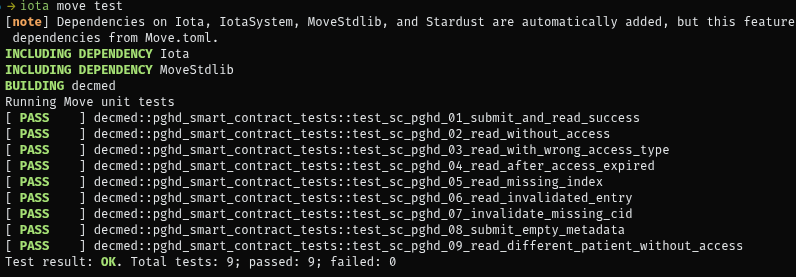
\includegraphics[width=\textwidth]{resources/chapter-4/pengujian_sc.png}
	\caption{Hasil Pengujian \textit{Smart Contract}}\label{fig:smart-contract-test-result}
\end{figure}


\begin{styledxltabular}{|>{\raggedright\arraybackslash}p{0.10\textwidth}|>{\raggedright\arraybackslash}p{0.22\textwidth}|>{\raggedright\arraybackslash}X|>{\raggedright\arraybackslash}p{0.26\textwidth}|>{\raggedright\arraybackslash}p{0.10\textwidth}|}
    \hiderowcolors
    \caption{Ekspektasi Balikan Pengujian \textit{Smart Contract} PGHD}\label{tab:expected-output-smart-contract} \\
    \hline
    \rowcolor{headerBg}
    \textbf{Kode} & \textbf{Skenario} & \textbf{Ekspektasi Hasil} & \textbf{Ekspektasi Balikan} & \textbf{Hasil} \\
    \hline
    \showrowcolors
    \endfirsthead
    \hline
    \rowcolor{headerBg}
    \textbf{Kode} & \textbf{Skenario} & \textbf{Ekspektasi Hasil} & \textbf{Ekspektasi Balikan} & \textbf{Hasil} \\
    \hline
    \endhead
    \hline
    \endfoot
    \hline
    \endlastfoot
    T-SC-01 & \textit{Submit} dan baca PGHD dengan akses valid. & Daftar PGHD berisi satu \textit{metadata} dan detail \textit{index} 0 dapat dibaca. & \texttt{PASS} & Sukses \\
    \hline
    T-SC-02 & Baca PGHD tanpa akses. & Akses ditolak karena \textit{access token} tidak ditemukan. & \texttt{EAccess\-NotFound} & Sukses \\
    \hline
    T-SC-03 & Baca PGHD memakai akses \textit{medical record}. & Akses ditolak karena tipe akses tidak sesuai dengan PGHD\@. & \texttt{EInvalid\-Access\-Type} & Sukses \\
    \hline
    T-SC-04 & Baca PGHD setelah akses \textit{expired}. & Akses ditolak karena melewati durasi akses yang diizinkan. & \texttt{EAccess\-Expired} & Sukses \\
    \hline
    T-SC-05 & Buka \textit{index} PGHD yang tidak ada. & Detail PGHD tidak dikembalikan karena \textit{index} tidak ditemukan. & \texttt{EPGHD\-Record\-NotFound} & Sukses \\
    \hline
    T-SC-06 & Buka entri PGHD yang \textit{invalid}. & Entri ditolak karena data sudah ditandai tidak valid. & \texttt{EPGHD\-Record\-Invalid} & Sukses \\
    \hline
    T-SC-07 & \textit{Invalidate} CID PGHD yang tidak ada. & Operasi invalidasi ditolak karena CID tidak ditemukan. & \texttt{EPGHD\-Record\-NotFound} & Sukses \\
    \hline
    T-SC-08 & \textit{Submit} \textit{metadata} PGHD kosong. & \textit{Metadata} tidak disimpan karena tidak memenuhi validasi minimum. & \texttt{EInvalid\-Pghd\-Metadata} & Sukses \\
    \hline
    T-SC-09 & Baca PGHD pasien berbeda. & Akses ditolak karena \textit{grant} akses tidak berlaku untuk pasien tersebut. & \texttt{EAccess\-NotFound} & Sukses \\
    \hline
\end{styledxltabular}
